\section{System Design}
\label{sec:system}

\subsection{Overall Architecture}
\label{sec:overall-architecture}

ZhuLong is built on Cline-CLI \cite{cline2024cline}, extended with EDA-specific retrieval, documentation, and execution capabilities. We call the resulting runtime an \textbf{ICL-type autonomous agent}: it decides its own next action, keeps no explicit posterior, and maintains its belief state implicitly by in-context learning (formalized in Section~\ref{sec:grounding-theory}). As shown in Figure~\ref{fig:architecture}, the system comprises three components---the LLM-based agent runtime, the API knowledge base, and the EDA execution environment---interacting through three MCP tools.

\begin{figure*}[t]
\centering
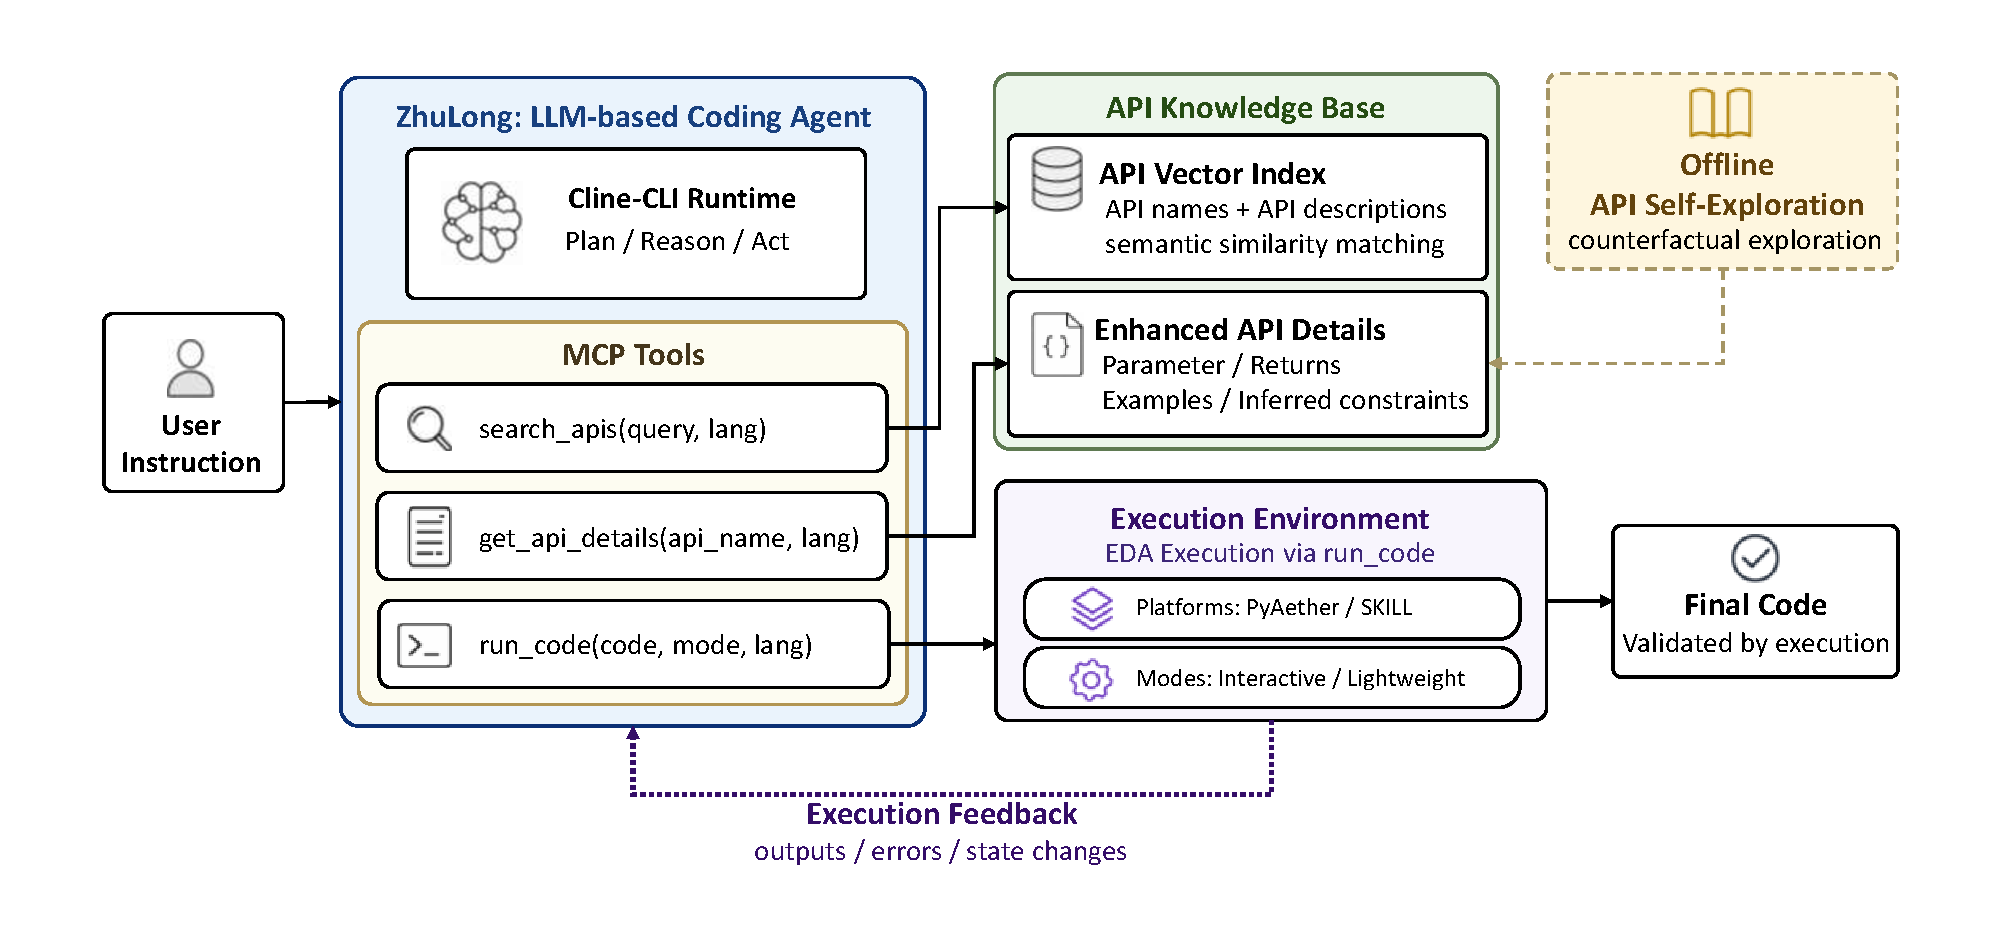
\includegraphics[width=0.9\textwidth]{figures/zhulong_arch_2.pdf}
\caption{ZhuLong system architecture. The agent interacts with API retrieval, documentation, and EDA execution via three unified MCP tools. Execution feedback supports iterative refinement.}
% ZhuLong系统架构。智能体通过三个统一的MCP工具与API检索、文档和EDA执行环境交互。执行反馈支持迭代优化。
\Description{Block diagram of ZhuLong's three components: the LLM agent runtime, the API knowledge base (search and retrieval), and the EDA execution sandbox. The runtime calls three MCP tools -- search_apis, get_api_details, and run_code -- with execution feedback looped back for iterative refinement.}
\label{fig:architecture}
\end{figure*}

\subsection{Three MCP Tools}
\label{sec:mcp-tools}

ZhuLong extends three MCP tools \cite{mcp2024protocol}, each accepting a unified \texttt{lang} parameter (\texttt{pyaether}, \texttt{skill}, or \texttt{tcl}) to support all three platforms with identical agent logic:
% ZhuLong扩展了三个MCP工具 \cite{mcp2024protocol}，每个工具接受统一的\texttt{lang}参数（\texttt{pyaether}或\texttt{skill}），以相同智能体逻辑支持两个平台：

\begin{itemize}
    \item \texttt{search\_apis(query, lang)} retrieves relevant APIs via semantic and keyword-based search. We index APIs by name and description using BGE-M3 embeddings \cite{bge2024} with FAISS \cite{douze2024faiss} for efficient similarity search, returning the top-$K$ results ($K=5$ by default) with confidence scores and descriptions.
    % \texttt{search\_apis(query, lang)}通过语义和关键词检索相关API。我们使用BGE-M3嵌入 \cite{bge2024}对API名称和描述建索引，FAISS \cite{faiss2017}支持高效相似度搜索，返回top-$K$结果（默认$K=5$），附带置信度分数和描述。
    
    \item \texttt{get\_api\_details(api\_name, lang)} fetches comprehensive documentation for a specified API, including parameter types, return values, and examples.
    % \texttt{get\_api\_details(api\_name, lang)}获取指定API的完整文档，包括参数类型、返回值和示例。
    
    \item \texttt{run\_code(code, mode, lang)} executes the generated code in the EDA environment. It supports two modes: (1) \textbf{lightweight}—runs in a sandboxed environment without a GUI session (standalone PythonE for PyAether, or SKILL in batch mode for Virtuoso), capturing outputs, errors, and state changes for iterative refinement; (2) \textbf{interactive}—runs inside an open EDA session via the agent-EDA bridge (socket communication), enabling operations on unsaved layouts and schematics.
    % \texttt{run\_code(code, mode, lang)}在EDA环境中执行生成的代码。支持两种模式：（1）\textbf{轻量模式}——在沙盒化环境中运行，无需GUI会话（PyAether使用独立PythonE环境，Virtuoso使用SKILL批处理模式），捕获输出、错误和状态变化供迭代优化使用；（2）\textbf{交互模式}——通过agent-EDA桥接（socket通信）在已打开的EDA会话内运行，支持操作未保存的版图和原理图。
\end{itemize}

\subsection{Agent Workflow}
\label{sec:agent-workflow}

The agent iteratively refines its output through execution feedback \cite{cline2024cline}. A typical trajectory reasons over the user instruction, retrieves APIs via \texttt{search\_apis}, inspects candidates via \texttt{get\_api\_details}, generates code, executes it via \texttt{run\_code}, observes the result, and re-plans---revising code, retrieving alternatives, or terminating---until success or further attempts are deemed unlikely. The agent is not constrained to a fixed sequence: it may skip retrieval when it already knows the required API, or conduct multiple retrieval rounds when initial results lack confidence.

